% =====================================================================
% 6.4 Excitação senoidal
% =====================================================================
\subsection{Excitação senoidal}

A Tabela~\ref{tab:seno} usa \(h=1~\mu\mathrm{s}\) e \(t_f=8~\mathrm{ms}\). A amplitude e a fase vêm do fasor da corrente. O erro da tabela é o maior erro absoluto da corrente ao longo de todo o intervalo, incluindo o transitório.

\begin{table}[htbp]
\centering
\caption{Fonte \(5\sin(\omega t)\) com \(R=20~\Omega\) e \(h=1~\mu\mathrm{s}\). Os erros estão em ampères. A fase toma a fonte como referência.}
\label{tab:seno}
\small
\setlength{\tabcolsep}{4pt}
\begin{tabular}{@{}lrrrrr@{}}
\toprule
Caso & \(|I|\) (mA) & Fase & Euler & Heun & RK4 \\
\midrule
\(\omega=\omega_0\) & 250{,}0 & \(0^{\circ}\) & \(1{,}31\times 10^{-2}\) & \(4{,}20\times 10^{-5}\) & \(2{,}09\times 10^{-10}\) \\
\(\omega=0{,}7\,\omega_0\) & 66{,}18 & \(+74{,}6^{\circ}\) & \(1{,}93\times 10^{-3}\) & \(6{,}42\times 10^{-6}\) & \(3{,}11\times 10^{-11}\) \\
\(\omega=1{,}4\,\omega_0\) & 70{,}00 & \(-73{,}7^{\circ}\) & \(2{,}88\times 10^{-3}\) & \(8{,}33\times 10^{-6}\) & \(4{,}58\times 10^{-11}\) \\
\bottomrule
\end{tabular}
\fonte{Elaborado pelos autores (2026).}
\end{table}

Na ressonância, a corrente cresce por alguns milissegundos até chegar a 250~mA, como mostra a Figura~\ref{fig:seno}. Abaixo da ressonância, em \(0{,}7\,\omega_0\), o circuito se comporta como capacitivo: a corrente se adianta \(74{,}6^{\circ}\) em relação à fonte, e a amplitude cai para 66,2~mA. Acima, em \(1{,}4\,\omega_0\), o circuito se comporta como indutivo: a corrente se atrasa \(73{,}7^{\circ}\), e a amplitude é 70,0~mA. O RK4 acompanha a solução exata com erro menor que \(10^{-9}\)~A. O Euler, no mesmo passo, erra cerca de 13~mA na ressonância, ou 5\% da amplitude permanente.

\begin{figure}[htbp]
\centering
\caption{Corrente com fonte senoidal de 5~V e \(h=1~\mu\mathrm{s}\). As retas tracejadas marcam a amplitude do regime permanente. O RK4 e a solução exata se sobrepõem.}
\label{fig:seno}
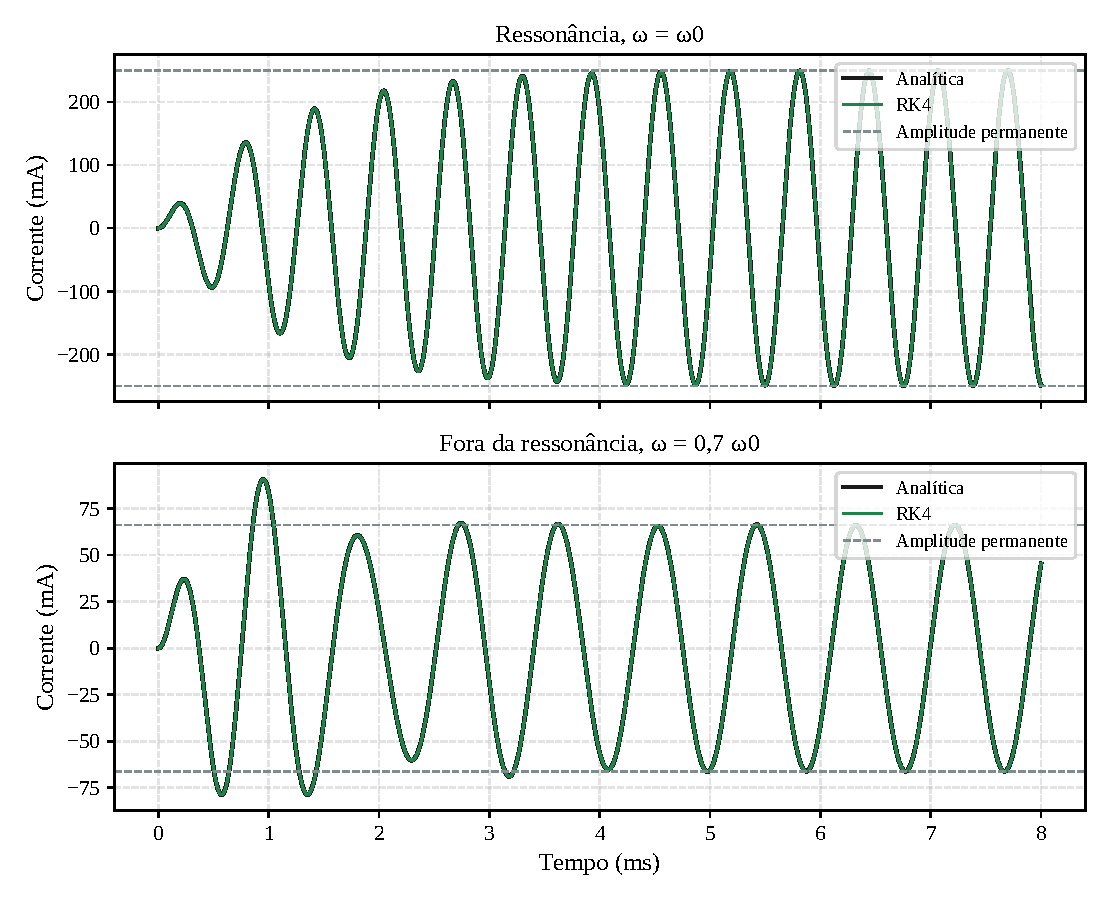
\includegraphics[width=\textwidth]{senoidal.pdf}
\fonte{Elaborado pelos autores (2026).}
\end{figure}

Para quem projeta um filtro, um erro de 5\% na amplitude já muda a leitura da seletividade. Com o mesmo passo, o RK4 entrega a resposta em frequência com erro desprezível.
